\documentclass[border=5pt]{standalone}
\usepackage{pgfplots}
\usepackage{tikz}
\usetikzlibrary{matrix}
\pgfplotsset{
  width=7cm,
  compat=1.15,
  /pgf/declare function= {
    w1(\x,\y,\z) = exp(-0.5 * (\y-4)^2);
   w2(\x,\y,\z) = exp(-0.5* \x^2); 
 },
}
\begin{document}
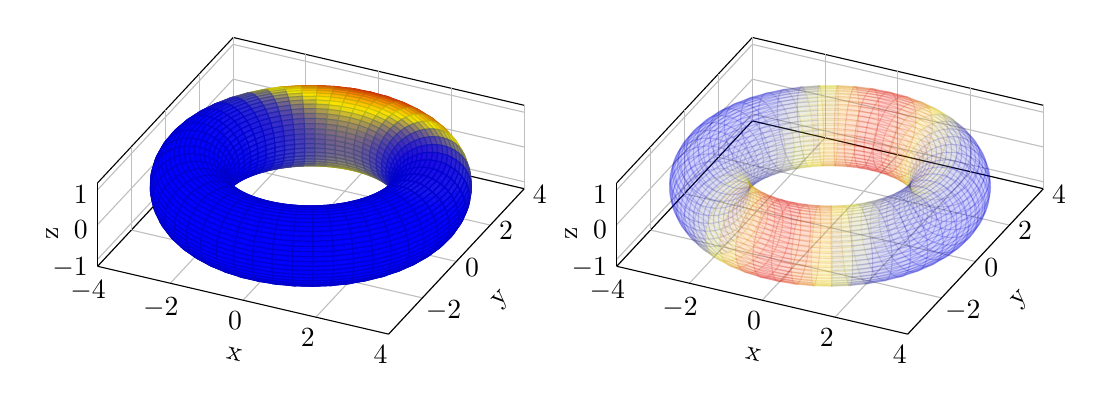
\begin{tikzpicture}
  \matrix {
  \begin{axis} [
      xlabel=x,
      ylabel=y,
      zlabel=z,
      xlabel style={sloped},
      ylabel style={sloped},
      zlabel style={sloped},
      xtick style={draw=none},
      ytick style={draw=none},
      ztick style={draw=none},
      unit vector ratio*=1 1 1,
      x tick label style={xshift=-0.0em},
      x label style={xshift=0.5em, yshift=0.5em},
      y tick label style={yshift=0.5em},
      y label style={yshift=0.5em, xshift=0.5em},
      z label style={yshift=-1.0em, xshift=0.5em},
      grid=major
    ]
     \addplot3[
         surf,
	 opacity=0.9,
         colormap/hot,
         samples=50,
         domain=0:2*pi,
         y domain=0:2*pi,
         z buffer=sort,
	 point meta={w1(x,y,z)}
       ]
       ( {(3+cos(deg(x)))*cos(deg(y+pi/2))}, 
         {(3+cos(deg(x)))*sin(deg(y+pi/2))}, 
         {sin(deg(x))}
       );
  \end{axis}
    &
  \begin{axis} [
      xlabel=x,
      ylabel=y,
      zlabel=z,
      xlabel style={sloped},
      ylabel style={sloped},
      zlabel style={sloped},
      unit vector ratio*=1 1 1,
      xtick style={draw=none},
      ytick style={draw=none},
      ztick style={draw=none},
      x tick label style={xshift=-0.0em},
      x label style={xshift=0.5em, yshift=0.5em},
      y tick label style={yshift=0.5em},
      y label style={yshift=0.5em, xshift=0.5em},
      z label style={yshift=-1.0em, xshift=0.5em},
      grid=major
    ]
     \addplot3[
         surf,
	 opacity=0.1,
         colormap/hot,
         samples=50,
         domain=0:2*pi,
         y domain=0:2*pi,
         z buffer=sort,
	 point meta={w2(x,y,z)}
       ]
       ( {(3+cos(deg(x)))*cos(deg(y+pi/2))}, 
         {(3+cos(deg(x)))*sin(deg(y+pi/2))}, 
         {sin(deg(x))}
       );
  \end{axis}\\
  };
\end{tikzpicture}
\end{document}

